\newpage

\section{More Circles}

\fixnote{Move this first problem to the activity called ``Of Angles and Circles.''} 
\begin{prob}
Prove:  Given a chord of a circle, any inscribed angle defined by this chord is half the measure of the central angle defined by this
chord.  Hint:  Prove $m\angle AXB = \frac{1}{2}m\angle AOB$ for the sequence of cases below.  
$$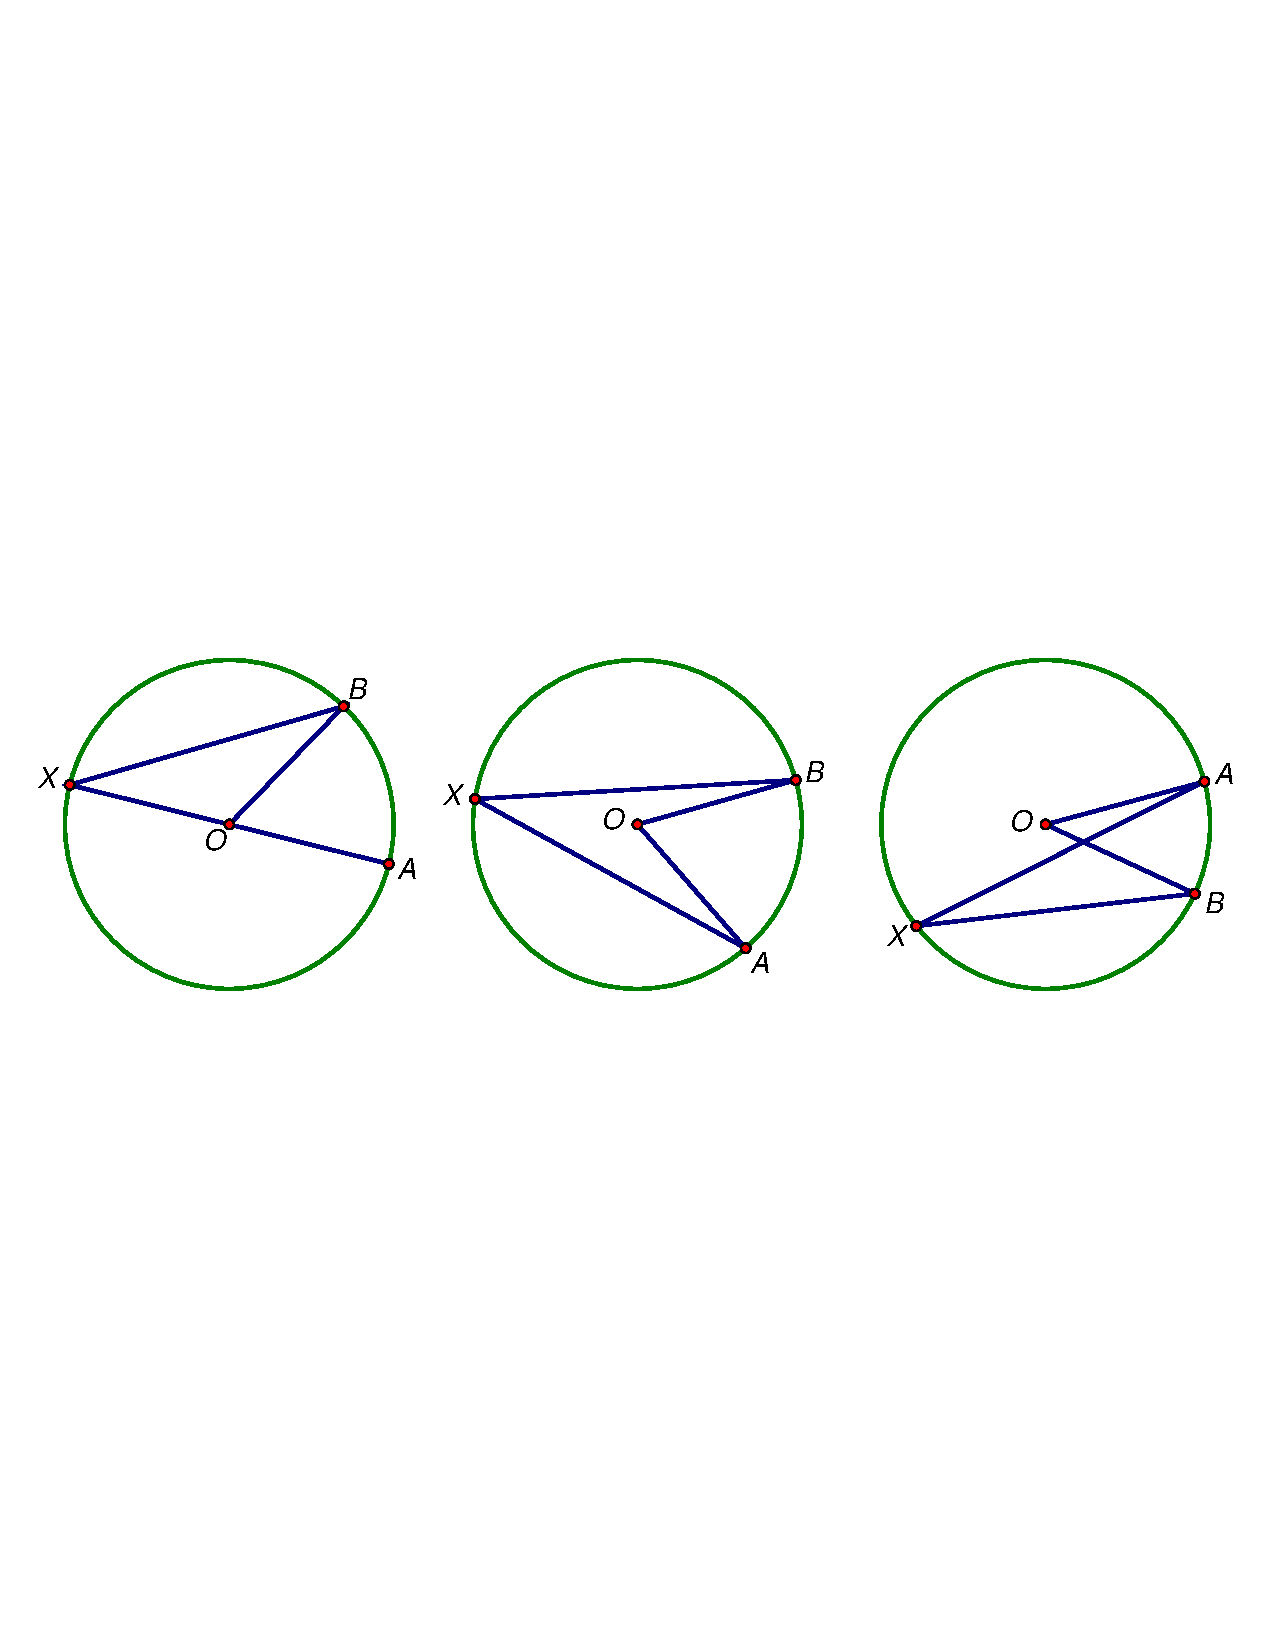
\includegraphics[width=3.5in]{InscribedAngle.pdf}$$
\end{prob}

\begin{prob}
Prove: The radius of a circle is perpendicular to the tangent where the radius intersects the circle.  Hint:  Suppose not. 
\end{prob}

\begin{prob}
Draw an angle that circumscribes a circle.  Find a relationship between the measure of the angle and the measure of the central angle intercepted by the same chord.
$$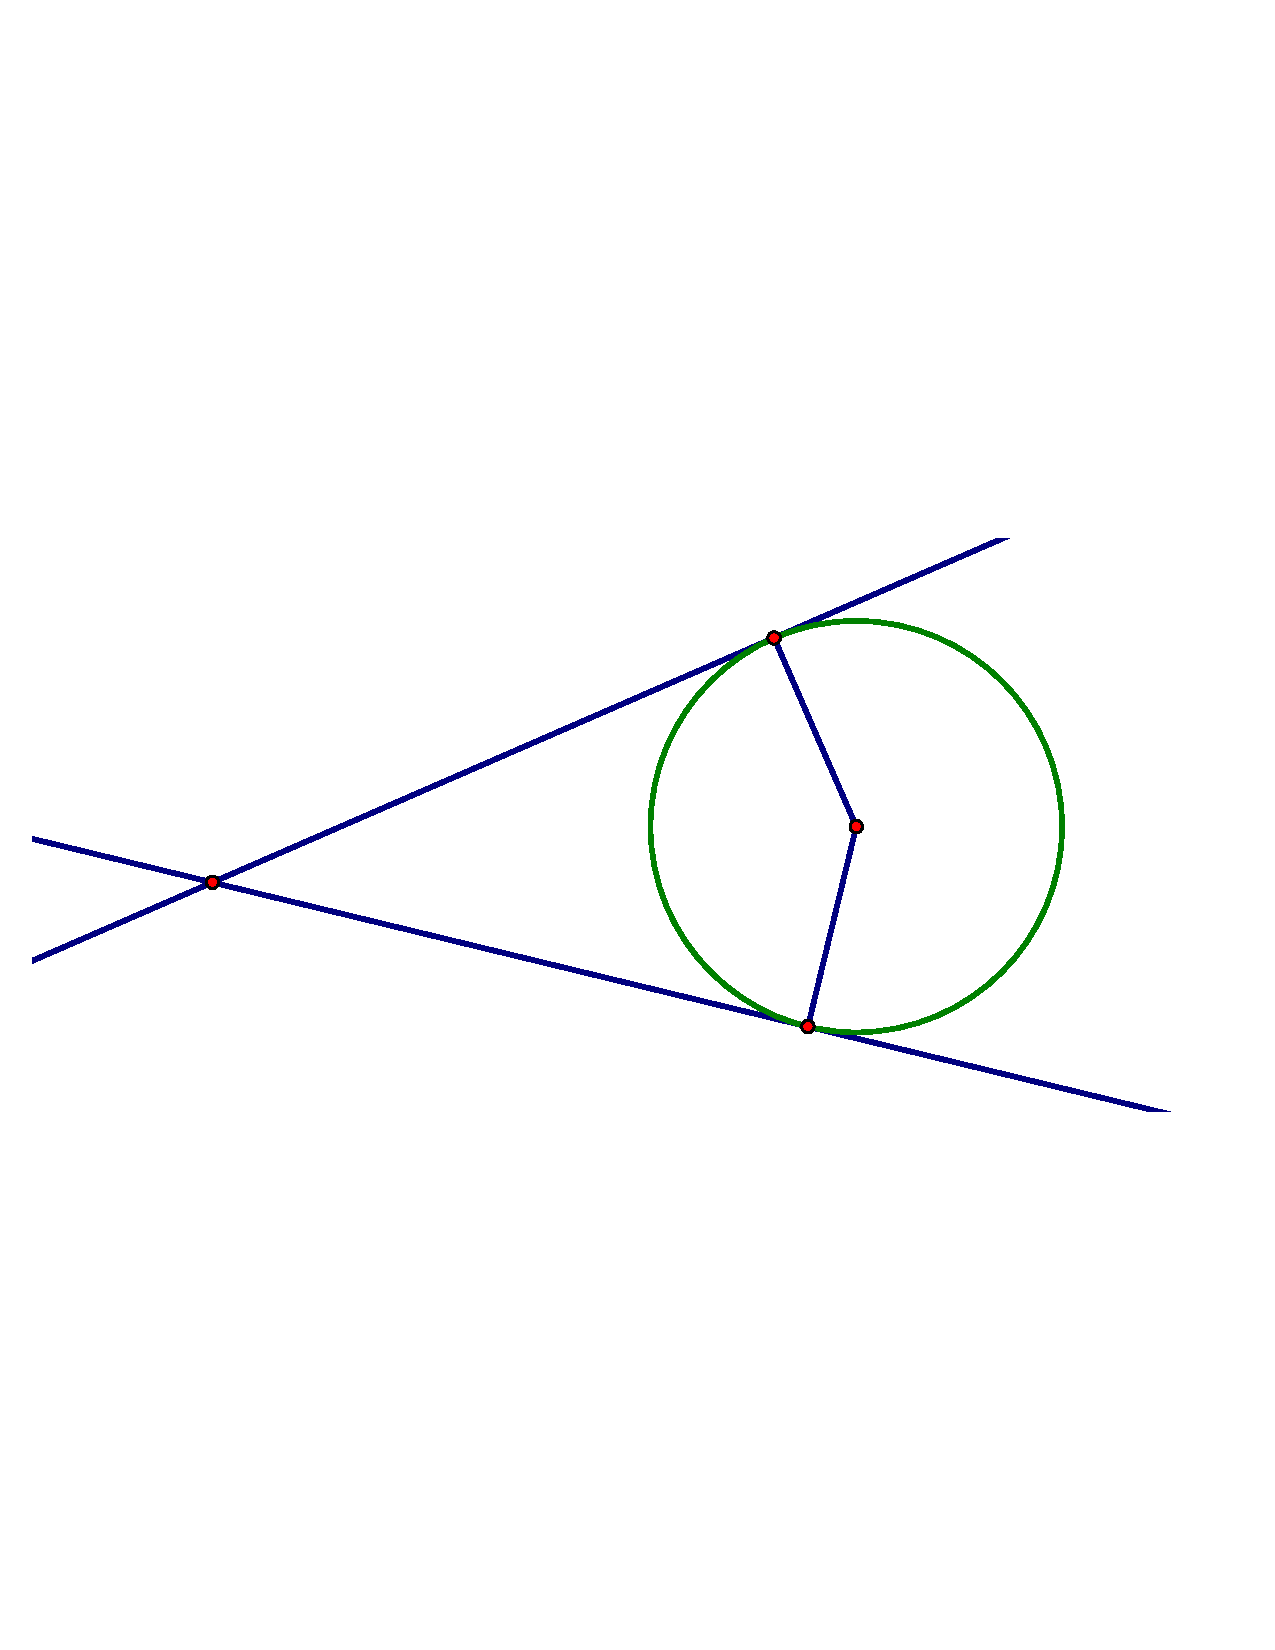
\includegraphics[width=2.5in]{CircumscribedAngle.pdf}$$
\end{prob}

\begin{prob}
Prove: A radius that is perpendicular to a chord bisects the chord. 
\end{prob}

\begin{prob}
Prove:  A radius that bisects a chord is perpendicular to the chord. 
\end{prob}

\begin{prob}
Show that, given any three non-collinear points in the Euclidean
plane, there is a unique circle passing through the three points.
\end{prob}

But how about four points in the plane, no three of which are collinear?

\begin{prob}
Draw four points in the Euclidean plane, no three of which are collinear, that cannot lie on a single circle.
\end{prob}

\begin{prob}
Using a compass, draw a large circle, and inscribe a quadrilateral in the circle.  Measure the four angles.  Repeat with another circle and quadrilateral.  What do you notice?  Identify a condition on any quadrilateral that is inscribed in a circle.  
\end{prob}

\begin{prob}
Construct a tangent line to a circle from a point outside the given circle.
$$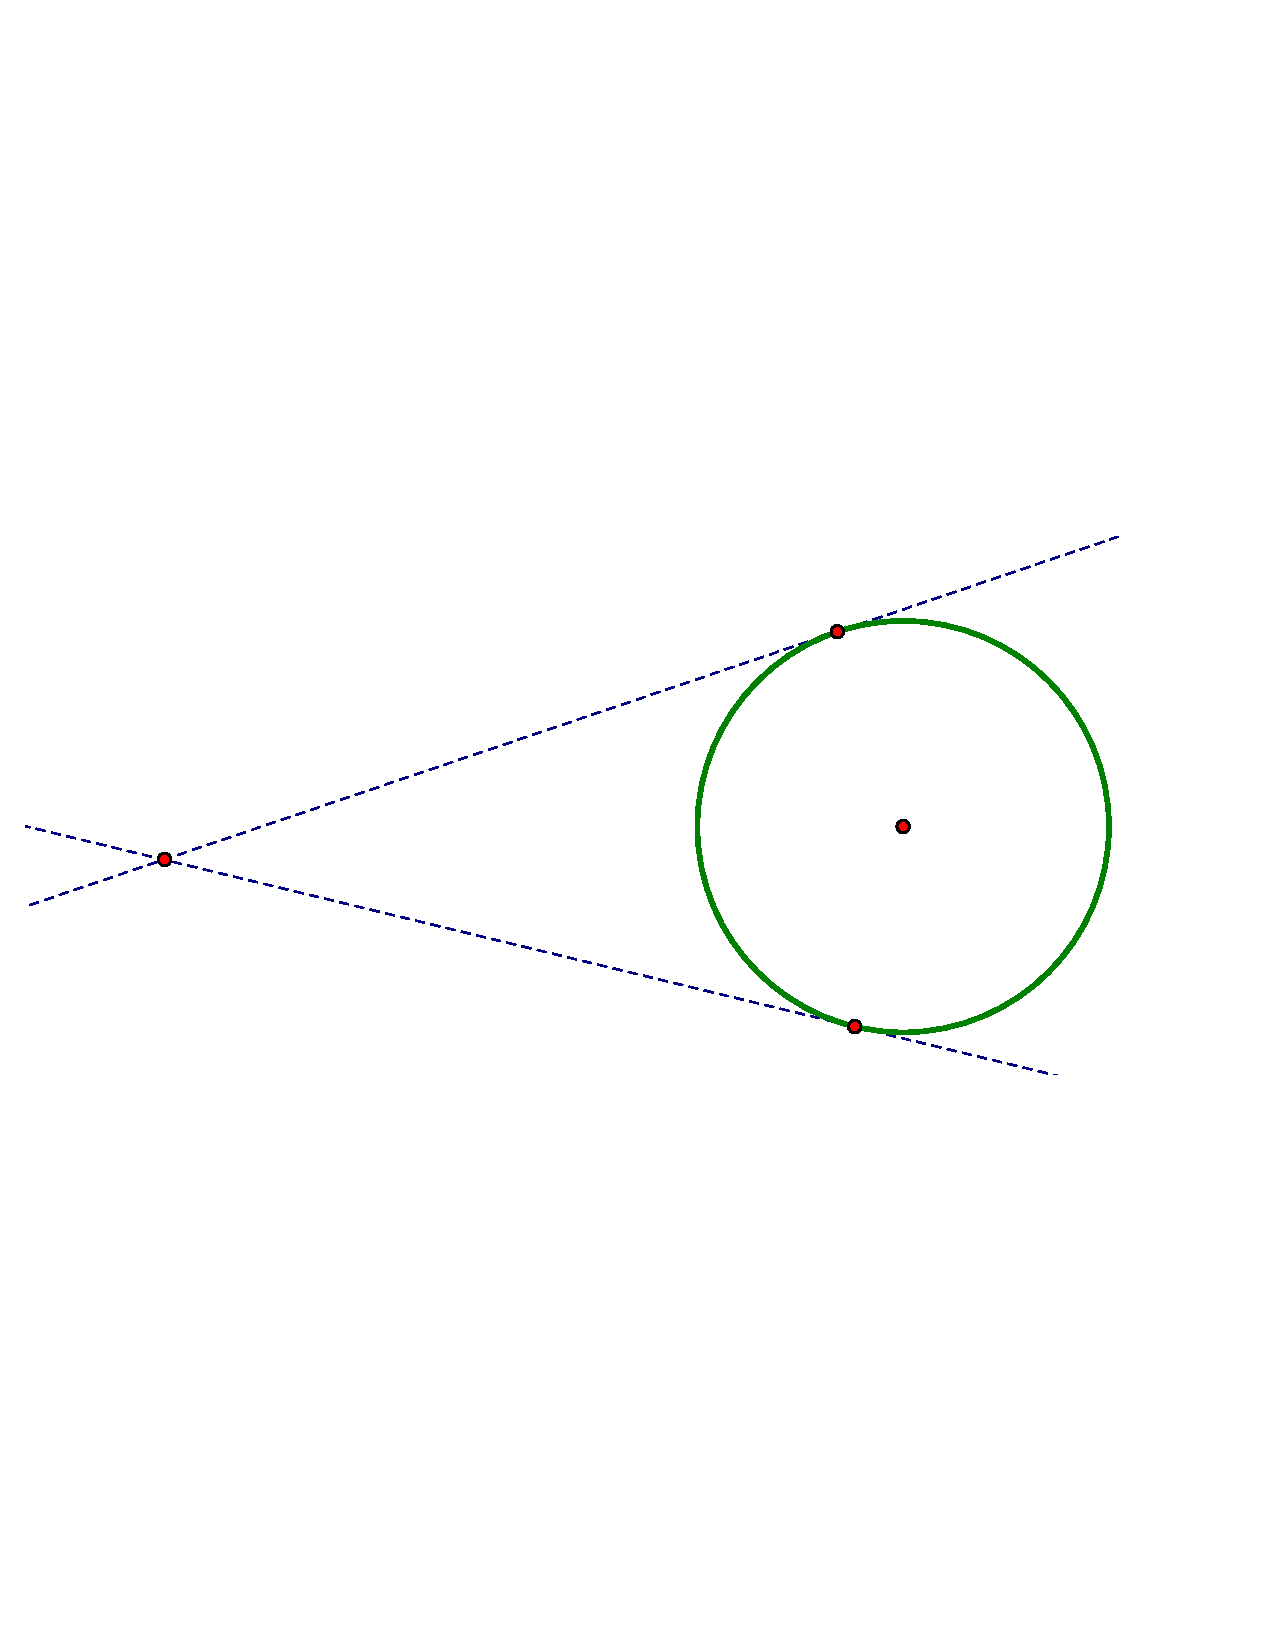
\includegraphics[width=3in]{Tangent.pdf}$$
\end{prob}

\begin{prob}
Give an informal derivation of the relationship between the circumference and area of a circle.  Imagine cutting a circle into ``pie pieces'' and rearranging the pieces into a shape like the one below.  As the circle is cut into more and more equal-sized ``pie pieces,'' what does the rearranged shape begin to resemble?  Can you find the area of this shape?  
$$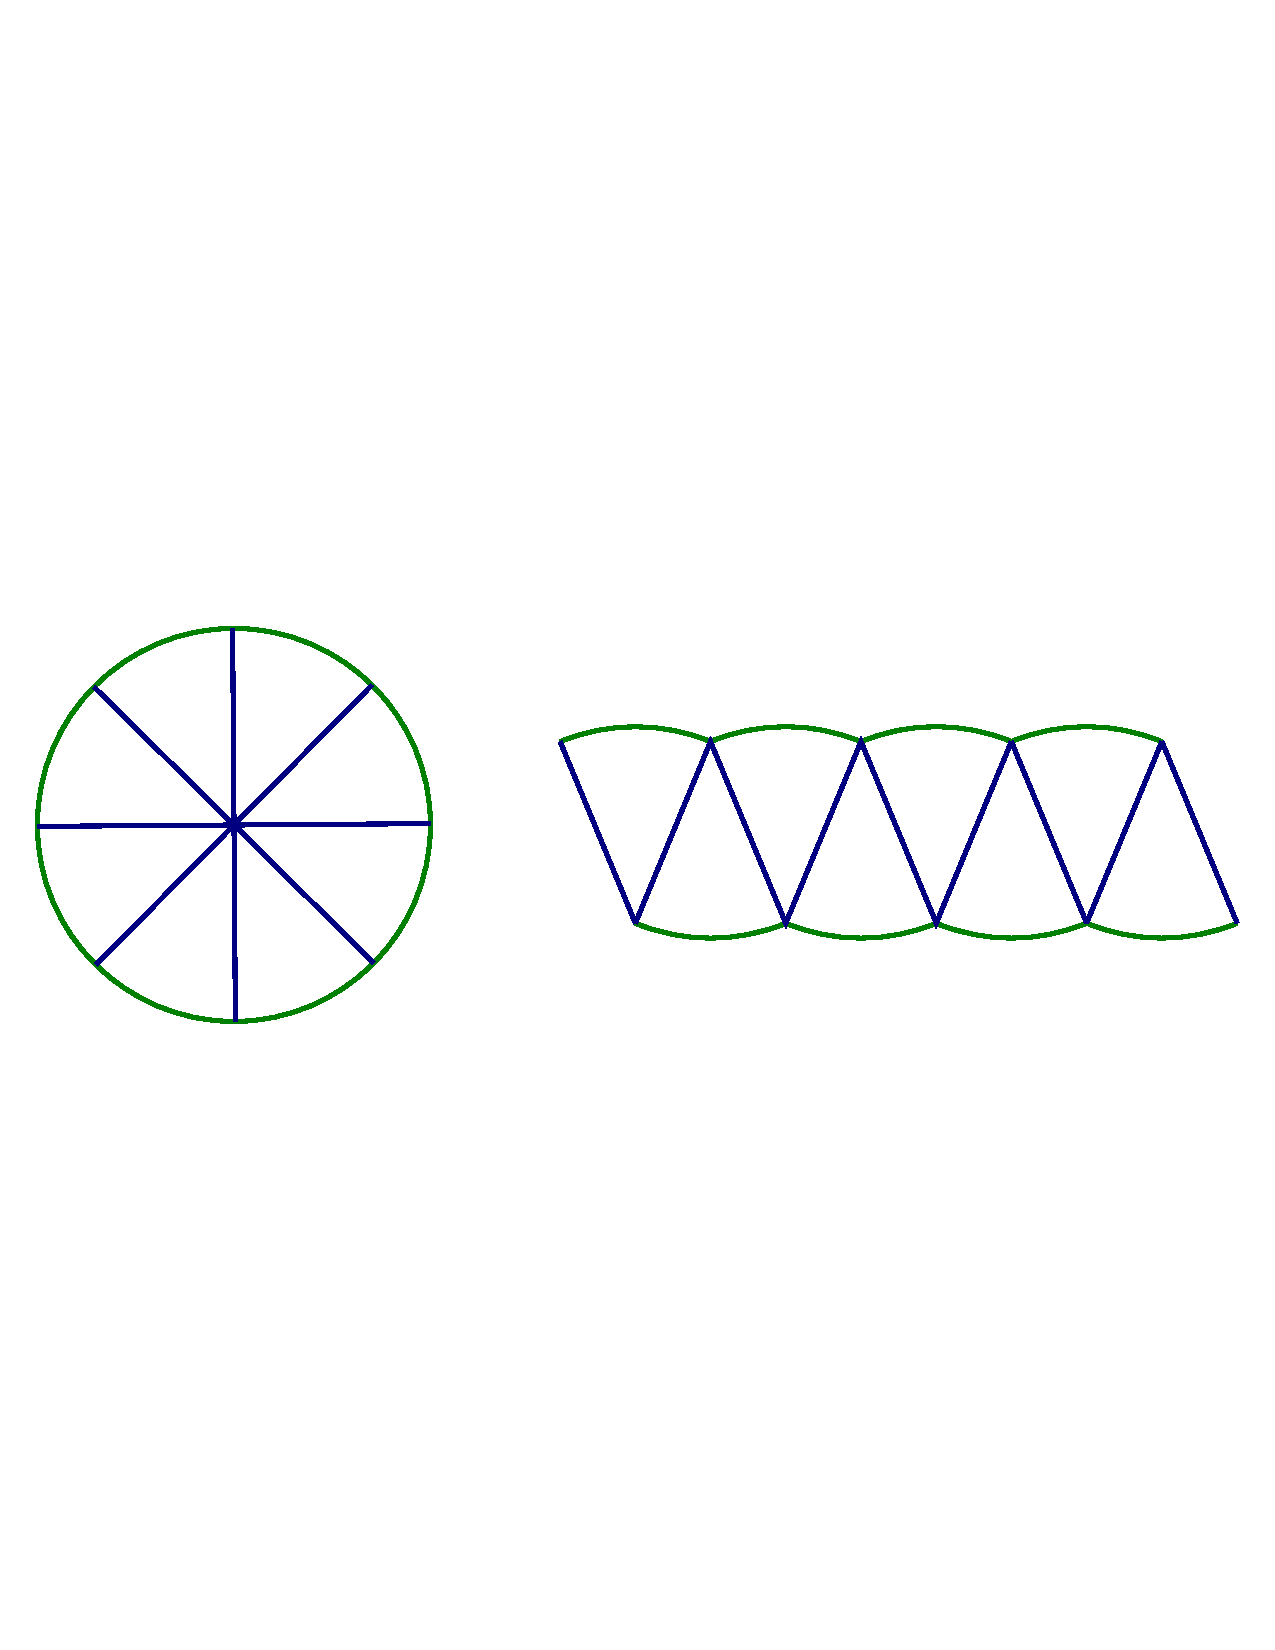
\includegraphics[width=3.5in]{CircleArea.pdf}$$
\end{prob}

\begin{prob}
Derive a formula for the length of the arc intercepted by an cenral angle of a circle.  
\end{prob}
%  is proportional to the radius, 
%  and define the radian measure of the angle as the constant of proportionality; 

\begin{prob}
Derive a formula for the area of a sector of a circle.  
\end{prob}







